\begin{lstlisting}
mq中现有支持的量子门:
1. 固定门
2. 含参门(如何与pr结合)
3. 自定义量子门
  a. 固定门
  b. 含参门(支持任意多比特,通过numba编译,JIT)

基本使用方法:
1. on方法
2. 强调所有门都可任意加控制比特
\end{lstlisting}


\maketitle
%%%%%%%%%%%%%%%%%%%%%%%%%%%%%%%%%%%%%%%%%%%%%%%%%%%%%%%%%%%%%%%%%%%%%%%%
\subsubsection{Quantum Gates}
Similar to how a classical computer is made up of classical circuits and classical bits,a quantum computer is made up of quantum circuits and qubits.In quantum circuits,quantum gates(quantum logic gates) can perform state transitions with several qubits.They are basis of quantum circuits and have many important functions.\\
Unlike classical circuit logic gates,all quantum gates are reversible,and all classical gate operations can be implemented with quantum gates.All quantum gates can be represented by a unitary matrix,whose dimension is determined by the number of qubits it operated on.According to the number of bits operated,it can be divided into single quibt gates and multi-qubit gates.According to whether the initialization method in mindquantum contains parameters,it can be divided into None Parameter Gates and Parameter Gates.

\subsubsection{Basic None Parameter Gate}
Similar to logic gates in classical circuits, the transition of a quantum circuit state can be achieved through quantum gates. Any quantum gate can be represented by a matrix, the only limitation being that its matrix representation U is a unitary matrix, i.e. ${UU^{\dagger}=I}$.
At the same time, any unitary matrix can define a valid quantum gate, and the dimension of the matrix depends on the number of qubits it operates on.\\
Here are some examples of single qubit gates,let $\ket{\phi}=a\ket{0}+b\ket{1}$.\\
\begin{align*}
I\ket{\phi}&=\begin{bmatrix}
1 && 0\\
0 && 1
\end{bmatrix}\begin{bmatrix}
    a\\
    b
\end{bmatrix}=\begin{bmatrix}
    a\\
    b
\end{bmatrix} % I
\\
X\ket{\phi}&=\begin{bmatrix}
0 && 1\\
    1 && 0
\end{bmatrix}\begin{bmatrix}
    a\\
    b
\end{bmatrix}=\begin{bmatrix}
    b\\
    a
\end{bmatrix} % X
\\
Y\ket{\phi}&=\begin{bmatrix}
    0 && -i\\
    i && 0
\end{bmatrix}\begin{bmatrix}
    a\\
    b
\end{bmatrix}=\begin{bmatrix}
    -bi\\
    ai
\end{bmatrix} % Y
\\
Z\ket{\phi}&=\begin{bmatrix}
    1 && 0\\
    0 && -
\end{bmatrix}\begin{bmatrix}
    a\\
    b
\end{bmatrix}=\begin{bmatrix}
    a\\
    -b
\end{bmatrix} % Z
\\
H\ket{\phi}&=\frac{1}{\sqrt{2}}\begin{bmatrix}
    1 && 1\\
    1 && -1
\end{bmatrix}\begin{bmatrix}
    a\\
    b
\end{bmatrix}=\frac{1}{\sqrt{2}}\begin{bmatrix}
    a+b\\
    a-b
\end{bmatrix} % H
\end{align*}

\subsubsection{Basic Parameter Gate}
Pauli matrices are the most important matrices, and they form a set of bases for spatial operators. When the Pauli matrix appears on the exponents, three classes of useful unitary operators are produced, namely rotation operators with respect to $\hat{x}, \hat{y}, \hat{z}$, defined by the following equation.\\
\begin{align*}
Rx(\theta)&=e^{-\frac{i\theta X}{2}}=\cos{\frac{\theta}{2}}I-i\sin{\frac{\theta}{2}}X=\begin{bmatrix}
        \cos{\frac{\theta}{2}} && -i\sin{\frac{\theta}{2}}\\
        -i\sin{\frac{\theta}{2}} && \cos{\frac{\theta}{2}}
    \end{bmatrix} % RX
\\
Ry(\theta)&=e^{-\frac{i\theta Y}{2}}=\cos{\frac{\theta}{2}}I-i\sin{\frac{\theta}{2}}Y=\begin{bmatrix}
    \cos{\frac{\theta}{2}} && -\sin{\frac{\theta}{2}}\\
    \sin{\frac{\theta}{2}} && \cos{\frac{\theta}{2}}
    \end{bmatrix} % RY
\\
Rz(\theta)&=e^{-\frac{i\theta Z}{2}}=\cos{\frac{\theta}{2}}I-i\sin{\frac{\theta}{2}}Z=\begin{bmatrix}
    e^{\frac{-i\theta}{2}} && 0\\
    0 &&  e^{\frac{i\theta}{2}}
    \end{bmatrix} % RY
\end{align*}
    

Since there are an infinite number of 2*2 matrices, the number of quantum gates is also infinite. According to the Z-Y decomposition, a unitary matrix U over any single qubit can be represented as $U=e^{i\alpha}Rz(\beta)Ry(\gamma)Rz(\delta)$.\\
Therefore, in order to construct arbitrary quantum gates, it is necessary to use parameters to construct rotating gates. There are three initialization methods provided in mindquantum, because Parameter Resolver has three initialization methods. \\
Take the RX gate as an example:
\begin{lstlisting}
from mindquantum.core.gates import RX
import numpy as np

rx1 = RX(0.5)
rx2 = RX('a')
rx3 = RX({'a': 0.2, 'b': 0.5})
print('rx1 is expressed as:{}\nThe matrix of rx1 is{}'.format(rx1, np.round(rx1.matrix(),3)))
print('rx2 is expressed as:{}\nThe matrix of rx2 is{}'.format(rx2, np.round(rx2.matrix({'a': 0.1}),3)))
print('rx3 is expressed as:{}\nThe matrix of rx3 is{}'.format(rx3, np.round(rx3.matrix({'a': 1, 'b': 2}),3)))
\end{lstlisting}
Output:
\begin{lstlisting}
rx1 is expressed as:RX(1/2)
The matrix of rx1 is[[0.969+0.j    0.   -0.247j]
 [0.   -0.247j 0.969+0.j   ]]
rx2 is expressed as:RX(a)
The matrix of rx2 is[[0.999+0.j   0.   -0.05j]
 [0.   -0.05j 0.999+0.j  ]]
rx3 is expressed as:RX(1/5*a + 1/2*b)
The matrix of rx3 is[[0.825+0.j    0.   -0.565j]
 [0.   -0.565j 0.825+0.j   ]]
\end{lstlisting}

\subsubsection{Custom Quantum Gate}
Since it is difficult to construct arbitrary quantum gates by using general gates in practical applications, two methods for constructing custom quantum gates are provided in mindquantum. They are quantum gates without parameters and quantum gates with parameters.
\subsubsection{Universal Math Gate}
If the matrix representation of a gate is known, it is convenient to construct the gate in mindquantum. Two parameters are required to initialize UnivMathGate, which are the gate name and the matrix value. If the matrix is not unitary, the result cannot be normalized.
Example:
\begin{lstlisting}
from mindquantum.core.gates import UnivMathGate
import numpy as np

x_mat=np.array([[0,1],[1,0]])
X_gate=UnivMathGate('X',x_mat)
x1=X_gate.on(0,1)
print(x1)
\end{lstlisting}
Output:
\begin{lstlisting}
X(0 <-: 1)
\end{lstlisting}

\subsubsection{Universal Parameterized Gate}
Sometimes we need to construct a parameterized gate in which the parameter is self-defined.In mindqantum, this initialization method is provided,and its usage is basically as same as that of RX gate.Two parameters are required to initialize such a gate.One is a function or method to use only one parameter(similar to theta in RX) to generate a unitary matrix,noting that no error is reported if the resulting matrix is not unitary..The other is the function or method that produces the derivative of this matrix,which is used to calculate the gradient. This method supports the generation of arbitrary qubit operators and can accelerate the performance by numba.JIT.
Example:
\begin{lstlisting}
from mindquantum.core.circuit import Circuit
from mindquantum.core.gates import gene_univ_parameterized_gate


def matrix(theta):
    return np.array([[np.exp(1j * theta), 0],
                     [0, np.exp(-1j * theta)]])


def diff_matrix(theta):
    return 1j * np.array([[np.exp(1j * theta), 0],
                          [0, -np.exp(-1j * theta)]])


TestGate = gene_univ_parameterized_gate('Test', matrix, diff_matrix)
circ = Circuit().h(0)
circ += TestGate('a').on(0)
print(circ)
print(TestGate(0).matrix())
print(circ.get_qs(pr={'a': 1.2}))
\end{lstlisting}
Output:
\begin{lstlisting}
q0: ──H────Test(a)──
[[1.+0.j 0.+0.j]
 [0.+0.j 1.-0.j]]
[0.25622563+0.65905116j 0.25622563-0.65905116j]
\end{lstlisting}

\subsubsection{On Method}
In quantum circuits, controlled operation is very common. Let U be any single qubit unitary operation, then the controlled U operation is a double qubit operation. One is the control bit and one is the target bit. In mindquantum, we can implement this function through the on method. This method takes two parameters. One is the target bit and the other is the control bit, both of which can be single qubit or multi-qubits.It is worth emphasizing that any gate can add arbitrary control operations.\\
Example:
\begin{lstlisting}
from mindquantum.core.gates import X

x = X.on(0, [1,2])
print('Target qubit:{},Control qubits:{}'.format(x.obj_qubits,x.ctrl_qubits))
\end{lstlisting}
Output:
\begin{lstlisting}
Target qubit:[0],Control qubits:[1, 2]
\end{lstlisting}

\subsubsection{Controlled Method}
In addition to the on method, we can also add control bits via the Control method.The controlled method is used to add control qubits (which can be multiple) to any quantum circuit or quantum operator.\\
For example, we build a quantum circuit containing only two qubits and add a control qubit - q2 to it by controlled method:
\begin{lstlisting}
from mindquantum.algorithm.library import qft
from mindquantum.core.circuit import controlled

u1 = qft(range(2))
u2 = controlled(u1)(2)
u3 = controlled(u1)
u4 = u3(2)
u2.svg(),u3.svg()
\end{lstlisting}
By looking at the circuit diagram of u2 and u4, we can see that the results are the same.\\
In addition, we can add control bits to quantum circuits in batches. For example, in the following example, we add control bits to q0 and q1 - q2 and q3, respectively:
\begin{lstlisting}
u = controlled(qft)
u = u([2, 3], [0, 1])
u.svg()
\end{lstlisting}
\begin{figure}[h]
    \centering
    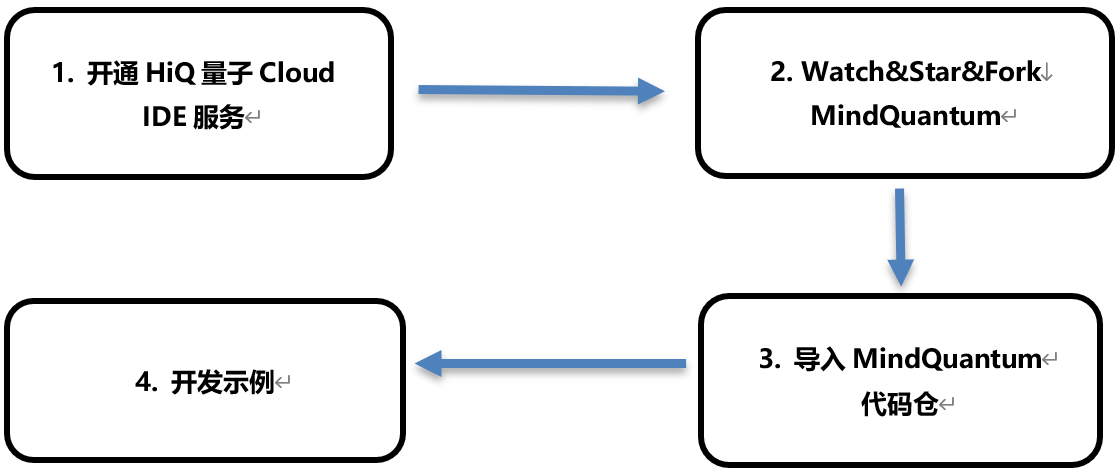
\includegraphics[width=0.5\linewidth]{1.png} % 插入svg出了点问题
    \caption{1.svg}
    \label{fig:enter-label}
\end{figure}

\end{document}
